\subsubsection{Alarm-history}

\begin{center}
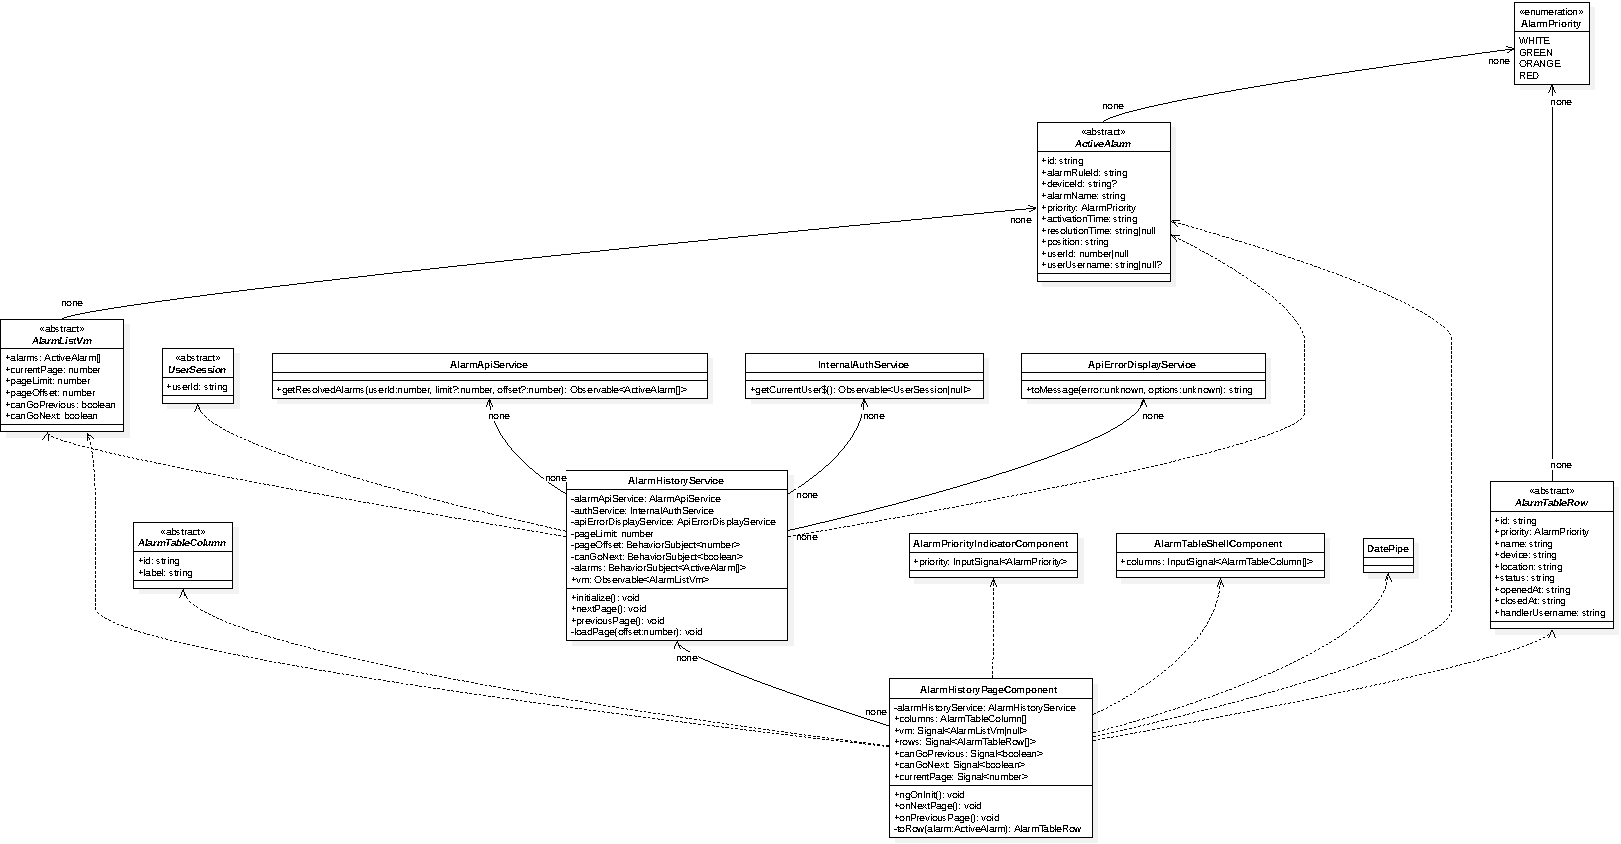
\includegraphics[width=\textwidth]{./frontend/alarm-history/alarm-history.pdf}
\captionof{figure}{Diagramma delle classi del modulo Alarm-history}
\end{center}

\addAtr{-}{alarmHistoryService: AlarmHistoryService}{Servizio utilizzato per il caricamento e la gestione dello storico degli allarmi.}
\addAtr{+}{columns: readonly AlarmTableColumn[]}{Lista delle colonne della tabella storico allarmi con i relativi identificativi ed etichette.}
\addAtr{+}{vm: Signal$<$AlarmListVm $|$ null$>$}{Segnale derivato dallo stream del view model del servizio storico allarmi.}
\addAtr{+}{rows: Signal$<$AlarmTableRow[]$>$}{Segnale calcolato che trasforma gli allarmi del view model in righe della tabella, ordinate per data di risoluzione decrescente.}
\addAtr{+}{canGoPrevious: Signal$<$boolean$>$}{Segnale calcolato che indica se è possibile navigare alla pagina precedente.}
\addAtr{+}{canGoNext: Signal$<$boolean$>$}{Segnale calcolato che indica se è possibile navigare alla pagina successiva.}
\addAtr{+}{currentPage: Signal$<$number$>$}{Segnale calcolato che restituisce il numero della pagina corrente.}
\addMet{+}{ngOnInit() : void}{Inizializza il servizio storico allarmi al momento della creazione del componente.}
\addMet{+}{onNextPage() : void}{Delega al servizio storico la navigazione alla pagina successiva degli allarmi.}
\addMet{+}{onPreviousPage() : void}{Delega al servizio storico la navigazione alla pagina precedente degli allarmi.}
\addMet{-}{toRow(alarm: ActiveAlarm) : AlarmTableRow}{Trasforma un allarme attivo nella corrispondente riga della tabella, normalizzando i valori assenti con valori di fallback.}
\makeCl{AlarmHistoryPageComponent}{Componente Angular che rappresenta la pagina dello storico degli allarmi, con supporto alla paginazione e visualizzazione delle informazioni di risoluzione. Le righe vengono ordinate per data di risoluzione decrescente e i valori assenti vengono sostituiti con valori di fallback.}

\addAtr{+}{alarms: ActiveAlarm[]}{}
\addAtr{+}{currentPage: number}{}
\addAtr{+}{pageLimit: number}{}
\addAtr{+}{pageOffset: number}{}
\addAtr{+}{canGoPrevious: boolean}{}
\addAtr{+}{canGoNext: boolean}{}
\makeAbCl{AlarmListVm}{Interfaccia che rappresenta il view model della lista degli allarmi, contenente i dati della pagina corrente e lo stato di navigazione della paginazione.}

\addAtr{+}{id: string}{}
\addAtr{+}{priority: AlarmPriority}{}
\addAtr{+}{name: string}{}
\addAtr{+}{device: string}{}
\addAtr{+}{location: string}{}
\addAtr{+}{status: string}{}
\addAtr{+}{openedAt: string}{}
\addAtr{+}{closedAt: string}{}
\addAtr{+}{handlerUsername: string}{}
\makeAbCl{AlarmTableRow}{Tipo che rappresenta una riga della tabella dello storico degli allarmi. Raccoglie le informazioni di priorità, posizione, stato e dati di risoluzione da visualizzare nella tabella.}

\addAtr{-}{alarmApiService: AlarmApiService}{Servizio utilizzato per le chiamate API relative agli allarmi risolti.}
\addAtr{-}{authService: InternalAuthService}{Servizio di autenticazione utilizzato per recuperare l'utente corrente.}
\addAtr{-}{apiErrorDisplayService: ApiErrorDisplayService}{Servizio utilizzato per la formattazione dei messaggi di errore provenienti dalle API.}
\addAtr{-}{pageLimit: number}{Numero massimo di allarmi visualizzabili per pagina.}
\addAtr{-}{pageOffset\$: BehaviorSubject$<$number$>$}{Subject che mantiene l'offset corrente della paginazione.}
\addAtr{-}{canGoNext\$: BehaviorSubject$<$boolean$>$}{Subject che mantiene la disponibilità di una pagina successiva.}
\addAtr{-}{alarms\$: BehaviorSubject$<$ActiveAlarm[]$>$}{Subject che mantiene la lista degli allarmi della pagina corrente.}
\addAtr{+}{vm\$: Observable$<$AlarmListVm$>$}{Stream reattivo che combina allarmi, offset e disponibilità della pagina successiva in un unico view model.}
\addMet{+}{initialize() : void}{Reimposta la paginazione e carica la prima pagina degli allarmi risolti.}
\addMet{+}{nextPage() : void}{Carica la pagina successiva degli allarmi risolti se disponibile.}
\addMet{+}{previousPage() : void}{Carica la pagina precedente degli allarmi risolti se l'offset corrente è maggiore di zero.}
\addMet{-}{loadPage(offset: number) : void}{Recupera gli allarmi risolti per l'utente corrente all'offset specificato, aggiornando la lista e lo stato di paginazione.}
\makeCl{AlarmHistoryService}{Servizio Angular per il caricamento e la gestione paginata dello storico degli allarmi risolti. Espone un view model reattivo che combina la lista degli allarmi e lo stato di paginazione per il consumo da parte dei componenti.}
